\chapter{Structure of the Experimental Setting}
\label{agent_code_chapter}
To train an agent on a specific environment, the user must utilize a command-line interface. There are various options available to cater to the user's needs. This chapter will outline all of the provided options and how they are encoded. However, we will first consider how the game represents discrete states.

\section{State}
The majority of the implemented agents in the game utilize the concept of state to facilitate learning. The agent will determine its next action based on the current state in which it finds itself. By dividing the game into discrete states, we are able to utilize tabular method algorithms to train an agent to play this continuous game. Once one obstacle is passed, the value of the state indicated refers to the next one. Each state is represented by a triplet consisting of distance, rotation, and next obstacle type. 

It is important to note that the game uses meters as the standard unit of distance measurement in Godot. This unit is used to represent the size, position, and movement of objects in the game world. It is worth mentioning that one meter in Godot is equal to the size of a standard cube. With that in mind, players can visualize Hans' approximate height of 12 meters and starting speed of 35 meters per second. Additionally, each tunnel in the game has a width and height of approximately 45 meters and a depth of 2800 meters.

The distance value indicates the distance of the agent from the next obstacle in meters. For example, if we set the \texttt{dists} parameter (indicated by the user, see \ref{opt:dists}) to 2, there are two possible distance values for the state: \textgreater 50, \textgreater 0, indicating that the agent is more than 50 meters away from the obstacle and at least 1-50 meter away from the obstacle, respectively. If the \texttt{dists} parameter is set to 1, the distance value remains constant at \textgreater 0. In the Chapter \ref{experiments_chapter} we will see that all types of environments in this game are able to learn when the \texttt{dists} parameter is equal to 1.  

The rotation parameter divides the obstacle circumference into \texttt{rots} number of intervals (see \ref{opt:rots}). As the tunnel rotates, the state label will indicate the rotation value to which Hans is aligned at the moment (in Figure \ref{fig:circumference} Hans is aligned with rotation value 240). If the \texttt{rots} parameter is set to 360, this would correspond to the number of degrees in a circle and result in 360 possible rotations. However, the obstacles in this game do not require such a high number of rotations and agents can be trained to avoid most obstacles using fewer than 10 rotations. 

\begin{figure}[h]
    \centering
    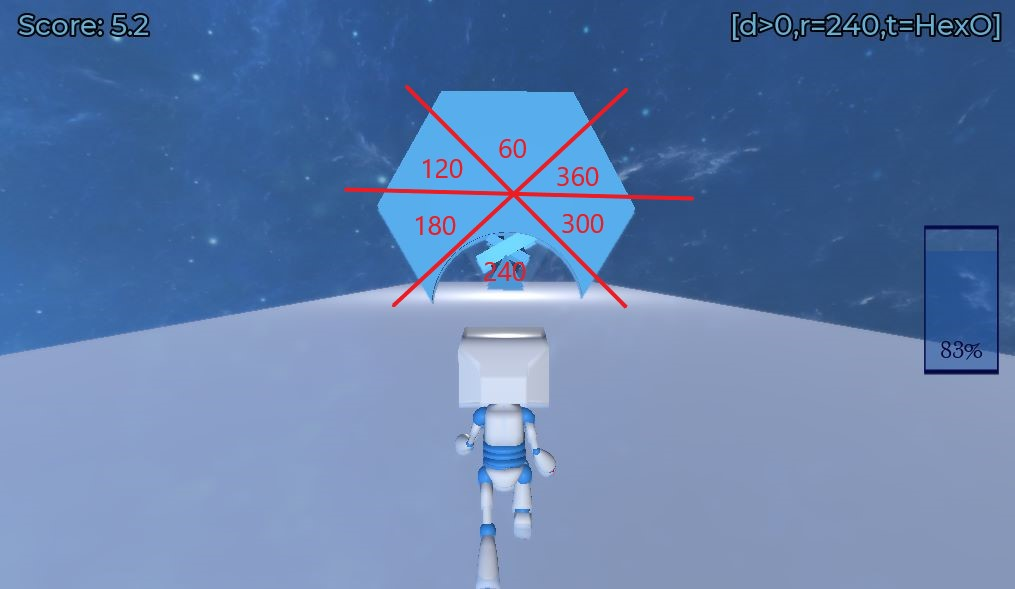
\includegraphics[width=\textwidth]{circumference}
    \caption{Rotations when \texttt{rots = 6}}
    \label{fig:circumference}
\end{figure}

Finally, the type parameter indicates the type of obstacle that Hans must avoid. Each obstacle has its own unique string representation, which allows the agent to learn to recognize the safe rotation for different types of obstacles. Using this information, along with the distance parameter, the agent can decide whether to move left, right, forward, or shoot in combination with any of these actions. To further explain this notion lets look back at the Figure \ref{fig:circumference}. At first glance, it may seem that a rotation of 240 would allow Hans to easily pass through the obstacle. However, upon closer inspection, it becomes clear that only a specific portion of the 240 rotation value is safe. The agent does not know the difference between being at any point of the 240 rotation and thus can easily make a fatal mistake. For this obstacle, indeed, there would be more \texttt{rots} needed in order for Hans to have at least one safe rotation value (meaning that the whole piece of the obstacle that rotation value covers is considered safe).

In Chapter \ref{experiments_chapter}, a noteworthy concept is presented where the agent can recognize a safe edge between two rotations, even if it is not provided with a completely safe rotation. By quickly shifting between these rotations, the agent is able to successfully navigate through the obstacle.

\section{Command line options}
\label{commOpt}
\begin{center}
\resizebox{\textwidth}{!}{%
\begin{tabular}{ | p{4cm}|p{10cm} | } 
  \hline
  \hyperref[opt:n]{n=int} & number of games\\ 
  \hline
  \hyperref[opt:stoppingPoint]{stoppingPoint=int} & stop after the agent wins this many consecutive games\\ 
  \hline
  \hyperref[opt:agent]{agent=string} & name of the agent\\ 
  \hline
  \hyperref[opt:level]{level=int} & number of the level to start from \\ 
  \hline
  \hyperref[opt:env]{env=[string]} & list of obstacles that will be chosen in the game \\ 
  \hline
  \hyperref[opt:shooting]{shooting=string} & enable or disable shooting  \\ 
  \hline
  \hyperref[opt:dists]{dists=int} & number of states in a 100-meter interval \\ 
  \hline
  \hyperref[opt:rots]{rots=int} & number of states in 360 degrees rotation \\ 
  \hline
  \hyperref[opt:agentSeedVal]{agentSeedVal=int} & seed value for the random moves the agent takes\\ 
  \hline
  \hyperref[opt:database]{database=string} & read the data for this command from an existing file and/or update the data after the command is executed  \\ 
  \hline
  \hyperref[opt:ceval]{ceval=bool} & performs continuous evaluation \\ 
  \hline
  \hyperref[opt:debug]{debug=bool} & display debug print statements \\ 
  \hline
  \hyperref[opt:options]{options} & displays options \\ 
  \hline
\end{tabular}}
\end{center}


\subsection{Command line option descriptions}
In this section, a more comprehensive clarification for the table presented earlier is provided. It is important to note that any of the options listed can be left out, as they all have default values assigned to them. In the event that no options are specified, a regular game with the \texttt{Keyboard} agent will be executed.

\subsubsection*{n}
\label{opt:n}
Number of games the agent will train on in this session. The default is 100.

\subsubsection*{stoppingPoint}
\label{opt:stoppingPoint}
If the agents manages to win this many consecutive games, the experiment is stopped. This is used to avoid long experiments if the agent has already learned the right policy and would simply keep winning. The default value is 25.

\subsubsection*{agent}
\label{opt:agent}
Name of the desired agent. \\
Options: [\texttt{Keyboard}, \texttt{Static}, \texttt{Random}, \texttt{MonteCarlo}, \texttt{SARSA}, \texttt{QLearning}, \\ \texttt{ExpectedSARSA}, \texttt{DoubleQLearning}]\\
Sub-options (only for the listed agents):
\texttt{MonteCarlo}, \texttt{SARSA}, \texttt{QLearning}, \texttt{ExpectedSARSA}, \texttt{DoubleQLearning}
=[float, float, float, float] :
[\texttt{gam} (range [0,1]), \texttt{eps} (range [0,1]), \texttt{epsFinal} (range [0,1]), \texttt{initOptVal} (range [0,$\infty$))]\\
Example usage: ``\texttt{agent=MonteCarlo:eps=0.1,gam=0.2}''\\
The meaning of the suboptions is explained in Chapter \ref{applied_algo_chapter}.

\subsubsection*{level}
\label{opt:level}
Number of the level to start from. Default value is 1.\\
Options: \texttt{[1, ... , 15]}\\
Note: after the 15th level, the agent is considered to have won the game.

\subsubsection*{env}
\label{opt:env}
List of obstacles that will be chosen in the game,\\
Options (any subset of): [\texttt{Traps}, \texttt{Bugs}, \texttt{Viruses}, \texttt{Tokens},
\texttt{I}, \texttt{O}, \texttt{MovingI}, \texttt{X}, \texttt{Walls}, \texttt{Hex},
\texttt{HexO}, \texttt{Balls}, \texttt{Triangles}, \texttt{HalfHex},
\texttt{Worm}, \texttt{LadybugFlying}, \texttt{LadybugWalking},
\texttt{Rotavirus}, \texttt{Bacteriophage}]\\
Note: if this parameter is not included, the environment will contain all available obstacles (i.e. the full game).\\
Example usage: ``\texttt{env=HexO,I,Bugs}''\\

\subsubsection*{shooting}
\label{opt:shooting}
Enable or disable shooting.\\
Options: [\texttt{enabled}, \texttt{disabled}, \texttt{forced}]\\
This option is disabled by default or if the environment does not have any bugs or viruses.

\subsubsection*{dists}
\label{opt:dists}
Number of states in a 100-meter interval.\\
This parameter is part of the state label and typical options range from 1 to 3. Default value is 1.

\subsubsection*{rots}
\label{opt:rots}
Number of states in 360 degrees rotation.
This parameter is part of the state label and the minimum viable option is 6. This is also the default value.

\subsubsection*{agentSeedVal}
\label{opt:agentSeedVal}
Seed value for the agent.\\
This parameter is used to produce multiple experiments with different random actions to verify if the agent can really learn under certain conditions or if it simply "to lucky" with the random moves.

\subsubsection*{database}
\label{opt:database}
Read or write data for this command from/to a file.\\
Options: [\texttt{read}, \texttt{write}, \texttt{read\_write}]\\
Note: these files are typically used to start another session of the agent's training from the last point of the previous session, to run a game with visuals and observe the agent's performance, or for plotting the results. This option does not affect the Keyboard, Static, or Random agents. Default option for this parameter is to neither read nor write.

\subsubsection*{ceval}
\label{opt:ceval}
Performs continuous evaluation.\\
This parameter indicates that after each training game, a test game will be played using only the policy(s) learned thus far. For example, if the user specifies ``n=100'', a total of 200 games will be executed, with 100 of them being training games and the remaining 100 being test games. This allows for the assessment of the agent's progress and performance during the training process. 
Options: [\texttt{true},\texttt{false} (default)]

\subsubsection*{debug}
\label{opt:debug}
Display debug print statements.
Options: [\texttt{true},\texttt{false} (default)]

\subsubsection*{options}
\label{opt:options}
Displays all of the mentioned options.


\subsection{Running the program}
There are several possibilities for running the game from the command line. In addition to various combinations of the options listed above, the user has the choice of running an experiment with or without the graphical interface. If they opt for the first possibility, the window will open and the game will be played at its normal speed. On the other hand, if the experiment is run without graphics, it will be over 200 times faster and the output will only be displayed in the terminal. This is achieved by a few things, mainly hiding the CSG geometry in every node. The computational power required to perform union, intersection, etc. on the CSG shapes is quite high and thus by not performing those calculations a game can run much faster. Of course, these shapes are not necessary for the experiments run without graphics, since the collision shapes are the ones that play a role in determining what happened in the game\footnote{The collision shapes refer to the shapes that are used to define the physical bounds of an object for the purpose of collision detection.}.
It is important to acknowledge that the experiments conducted in this study are entirely reproducible owing to the predetermined seed values for all the random variables. However, it should be noted that the values produced by a seed can differ across different versions of the Godot Engine. In order to obtain identical results to the experiments detailed in Chapter \ref{experiments_chapter}, it is recommended to use Godot Engine v3.2.3.stable.

To run the program in the command line, the user may benefit from adding the Godot executable to the PATH environment variable. This will allow them to start the application from the command line simply by entering the command \texttt{godot} while inside the same directory as the \texttt{project.godot} file.

By default, running the program in this manner will launch a normal game with the graphical interface and the \texttt{Keyboard} agent. However, the user can customize their experiment by using a combination of the options listed above. For example:

\begin{algorithm}
\begin{algorithmic}
\State godot database=write agent=SARSA:initOptVal=100.0,eps=0.3 env=HexO n=10 dists=1 rots=8
\end{algorithmic}
\end{algorithm}

Alternatively, the user may choose to train the agent faster by disabling the graphical interface and increasing the speed of the program. This can be achieved by modifying the previous command as follows:

\begin{algorithm}
\begin{algorithmic}
\State godot --no-window --fixed-fps 1 --disable-render-loop database=write agent=SARSA:initOptVal=100.0,eps=0.3 env=HexO n=10 dists=1 rots=8
\end{algorithmic}
\end{algorithm}

To view a list of available options, the user can simply enter the command \texttt{godot options}.

\section{Main}
The \texttt{Main.tscn} scene is the top level scene in the game and consists of a single Node type node. The script attached to this node, \texttt{Main.gd}, is responsible for ensuring that all options specified in the command line (as discussed in Section \ref{commOpt}) are executed correctly. This script is the starting point of the training and handles the initialization and execution of ore or more game sessions.
There are several key functions within the \texttt{Main.gd} script that are worth discussing in more detail.

\begin{center}
\line(1,0){400}
\begin{lstlisting}
func _ready():
	var unparsed_args = OS.get_cmdline_args()
	if unparsed_args.size() == 1 and unparsed_args[0] == "options":
		display_options()
		
	...	# parse args
	
	if set_param(args) == false:
    		display_options()
	else:
    		instance_agent()
    		build_filename()
    		if not agent_inst.init(...):
        		print("Something went wrong, please try again")
        		display_options()
    		play_game()
\end{lstlisting}
\line(1,0){400}
\end{center}

The \texttt{\_ready()} function is the starting point of the program when run from the command line. It is responsible for parsing all of the arguments and checking their validity. If any issues are encountered, the program will display options and terminate. If the arguments are valid, an agent will be instantiated and initialized. In cases where everything is in order, first game will be played by calling the \texttt{play\_game()} function.

\begin{center}
\line(1,0){400}
\begin{lstlisting}
func play_game():
	if agent == "Keyboard" and VisualServer.render_loop_enabled:
		... # play a regular game
	elif n > 0:
		n -= 1
		game = game_scene.instance()
		set_param_in_game()
		agent_inst.start_game(is_eval_game)
	else:
		agent_inst.save(write)
		print_and_write_ending()
\end{lstlisting}
\line(1,0){400}
\end{center}

The \texttt{play\_game()} function is called each time a game is played.Firstly, it will check if the agent selected was the \texttt{Keyboard} agent, and if so, the program will start one game session where the user has controls of Hans. Otherwise, one of the remaining agents will take over and play specified number of games (defined by the "n" parameter). If n games have already been played, the program will terminate after performing the last few tasks needed to save all of the knowledge gained form this particular session. Otherwise, a single game will be executed and number of games left decreased.

\begin{center}
\line(1,0){400}
\begin{lstlisting}
func on_game_finished(score, ticks, win, time):
	print_and_write_score(score, win)
	agent_inst.end_game(score, time)
	play_game()
\end{lstlisting}
\line(1,0){400}
\end{center}



The \texttt{game\_over()} function is called when the game emits a signal indicating that it has finished. Upon execution, this function outputs the necessary information, updates the agent through the \texttt{end\_game()} function, and then calls the \texttt{play\_game()} function to continue the game session.